
En este capítulo se describirán los métodos usados para llevar a cabo las simulaciones. 

Para realizar las simulaciones se utilizó el programa LAMMPS (Large-scale Atomic/Molecular Massively Parallel Simulator).
Es un software de código libre distribuido bajo los términos de GPL.
LAMMPS se caracteriza por hacer uso de las listas de vecinos [rapaport] para efecuar cálculos que permiten reducir la
complejidad algorítmica, permite correr las simulaciones en un único procesador o en paralelo (valíendose de técnicas de message-passing y descomposición espacial del dminio de simulación), además cuenta con una gran cantidad de funciones implementadas orientadas al uso de simulaciones de dinámica molecular. 

Todas las simulaciones constaron de N individuos en un recinto cuadrado cuyo tamaño estaba ligado a la cantidad de
peatones de modo tal que mantenga constante la densidad. En una de las paredes se ubicaron una o dos puertas. Las puertas se ubicaban simetricamente en el medio para evitar efectos de borde, cuando el recinto tenía dos salidas, ambas se fijaron del mismo ancho.
Para todas los sistemas estudiados se configuró un arreglo bidimensional de individuos, ordenados inicialmente tipo
red cuadrada, con una densidad de  0,6~personas/m$^2$, similar al límite de las regulaciones actuales~\cite{mysen}. Inicialmente todos los individuos tenían una velocidad aleatoria con una distribución gausiana centrada en cero.  Luego del instante inicial, los agentes cambiaban su velocidad acorde a la velocidad de deseo configurada 
de forma tal que los individuos evacúen por la puerta más cercana. Una vez que los individuos abandonaban el recinto no se los reinyectaba. De esta forma, al evacuar dejaban de importar sus observables. \\
La información era guardada cada 0,05~s. 
Para resolver la dinámica se utilizó el algoritmo de Verlet. 
Con el fin de compatibilizar el modelo de fuerza social con LAMMPS, se crearon varios módulos con las fuerzas que
caracterizan a este modelo. Todos estos fueron escritos en c++. En la siguiente sección se describe cada uno de ellos. 
%
%\begin{figure}[H]
%    \centering
%    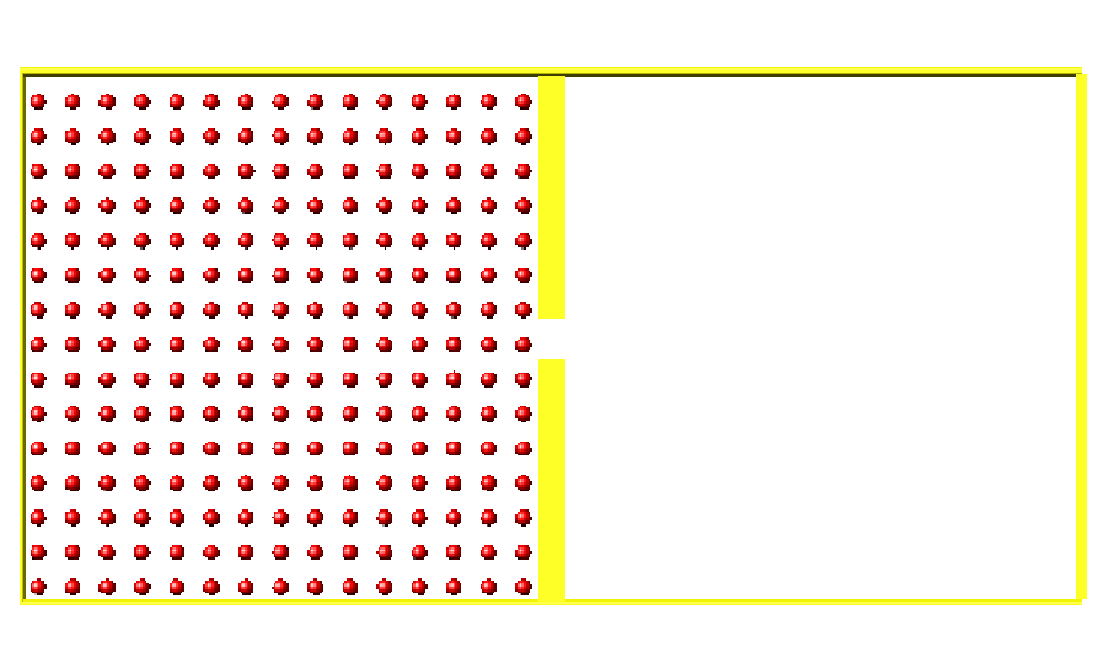
\includegraphics[scale=0.45]{figuras/0.eps}   
%    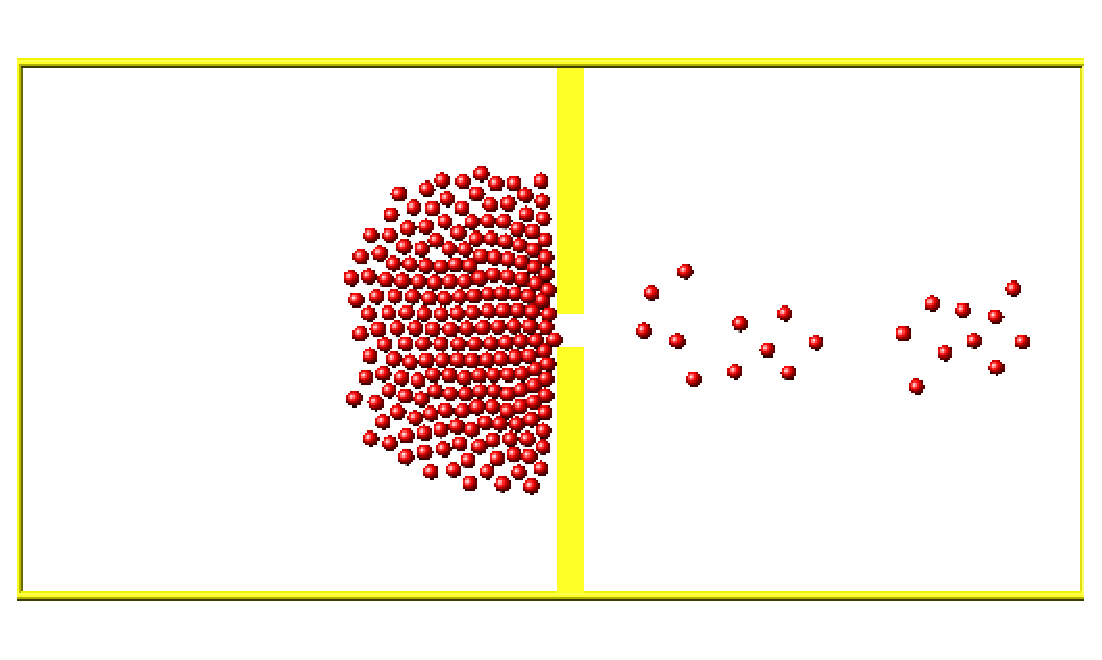
\includegraphics[scale=0.45]{figuras/500.eps}
%     \caption[width=5cm]{j}
%    \label{sim}
%\end{figure}

\section{Módulos}

{\Large pair\_social}

Este módulo se hizo para incluir la fuerza de repulsión social ($\mathbf{f}_s^{(ij)}$) del modelo de Helbing (ver sección 2.1). Toma como parámetros la constante B y la distancia de corte (si los individuos estan separados por una distancia mayor a este corte, la fuerza social entre ellos no se calcula).
Otros parámetros son agregados a través de la función pair\_coef. Estos son la constante A del modelo de Helbing, la distancia 
de corte y el radio de los individuos. Los valores utilizados fueron: A $=$ 2000, B$=$ 0,08 r\_cut $=$ 3,5 d $=$ 0,30.
La elección de la distancia de corte se tomó de modo tal que la fuerza social que sienten individuos separados a esa distancia
sea despreciable ($\sim$ 10$^{-12}$ N). El resto de los parámetros fueron extridos de la bibliografia del modelo de fuerza social~\cite{Helbing1}.

{\Large pair\_gran\_social}

Se creó para que exista rozamiento entre los individuos que están en contacto. Requiere como parámetro el valor de la constante de rozamiento, el mismo fue $\kappa =2,4 \times 10^5~kgm^{-1}s^{-1}$. Tanto el valor de $\kappa$ como la expresión de la fuerza concuerdan con los del modelo de Helbing.

{\Large fix\_wall\_social y fix\_wall\_gran}

Estos módulos son análogos a pair\_social y pair\_gran\_social pero aplicados a las fuerzas de interacción entre los individuos y las paredes. El primero simula la fuerza de repulsión y poseé los mismos parámetros que la repulsión entre individuos mientras que el segundo modela la fuerza de rozamiento dinámico. 

{\Large fix\_social\_self y fix\_social\_self\_multi}

La fuerza de deseo del modelo de Helbing fue simulada con estos módulos. El primero se usó para los recintos con una única puerta mientras que el segundo para recintos con dos. 
El primero requiere como parámetro la masa de los individuos y la velocidad de deseo. El target que tiene cada individuo, depende de la posición en donde se encuentre. Por cada puerta hay tres targets: superior, medio e inferior. El medio está ubicado en la mitad de la puerta, los otros 0,3 m por encima y por debajo.  Los individuos cuya posición en la coordenada 'y' sea mayor (menor) que el target superior (inferior) actualizan su velocidad para apuntar al target superior (inferior). Si se encuentran en medio de éstos, apuntan al centro de la puerta. De este modo los peatones siempre se dirigen al target más cercano.\\  
Cuando se simularon recintos con dos puertas se usó fix$\_$social$\_$self$\_$multi, sus parámetros son: la masa de los individuos, la velocidad de deseo y el gap (la distancia de separación entre puertas). Si el gap es nulo, las dos puertas estan unidas (formando una única puerta ancha). En este caso, se establecen tres targets: el superior (inferior), que está 0.3 m debajo (encima) del final de la puerta superior (inferior). Los individuos que se encuentran en el medio apuntan al centro (al igual que en el caso de una única puerta).
Si el gap no es nulo, es decir, existe una porción de pared entre ambas puertas, la dirección de la velocidad de los individuos se actualiza de forma análoga al caso de una puerta. De esta forma los individuos siempre buscan la salida más cercana. 

{\Large compute\_social\_pressure}

Calcula la función de presión social de la expresión \eqref{pv} despreciando el término cinético. Para cada timestep devuelve un vector con la pesión que soporta cada peatón como consecuencia de la interacción con sus vecinos. 

{\Large compute\_dijkstra\_atom}

Rotula con la misma etiqueta a todos los elementos que forman parte de un blocking cluster. Requiere como parámetro las posiciones en la coordenada 'y' de los puntos de origen y terminación del blocking cluster y la posición de la pared en la coordenada 'x'. Para cada timestep devuelve un vector con N componentes (siendo N la cantidad de peatones). Cada una de estas componentes esta asociada a un individuo; toma un número distinto de cero cuando el individuo forma parte de un cluster de bloqueo y cero en caso contrario. 

\section{Script básico}

A modo de ejemplo se describirá un script de lammps que se hizo para simular 225 individuos en un recinto de 20$\times$20~m con una puerta de 1,2~m. Este programa cuenta con dos ciclos {\tt for}, uno recorre diferentes valores de velocidad de deseo y el otro (anidado) sirve para tener 30 simulaciones con diferentes velocidades iniciales. \\
El programa devuelve un video de la simulación en formato mpg y un archivo txt con una tabla que indica: $v_d$, numero de iteración y el tiempo para el cual evacuaron más de 159 individuos.
El script está dividido en cinco partes: condiciones iniciales, fuerzas, evacuados, visualización y ejecución del proceso.\\ 
En las condiciones iniciales se fija la dimensión del problema (2d), las condiciones de contorno (no periódicas en las coordenadas x e y), el sistema de unidades usado (sistema intermacional), también se configuran los atributos de los individuos como el tamaño (60 cm diametro) y su peso (70~kg). La velocidad inicial se fijó con la funcion {\tt velocity}, la misma genera una distribución gausiana de velocidades que es asignada de forma aleatoria a los individuos. El módulo de la velocidad es 1,7~m/s. La semilla que genera la distribución de velocidades es el número de iteración.\\
En cuanto al tamaño de la región de simulación, se crearon tres zonas: la zona 1 es la que inicialmente poseé a los individuos (ordenados tipo red cuadrada separados 1,3~m entre si), la zona 2 es la región de evacuación y la zona 3 es la conexión entre ambas regiones (la puerta por donde pasan).\\
En la parte de fuerzas se especifican las interacciones que sienten los individuos y sus respectivos parámetros. La repulsión entre individuos (pair style social) utiliza la expresión $\ref{fsocial}$ con los parámetros: A=2000~N, B=0,08~m y se asignó un cutoff de 3,5~m. La fuerza granular (pair style gran/social) se basa en la fórmula $\ref{frozamiento}$ con $\kappa =2,4 \times 10^5~kgm^{-1}s^{-1}$. Se usaron los mismos parámetros para las expresiones análogas en la interacción individuo-pared (fix wall/region social y granular). La fuerza de deseo (fix social/self) tomó como parámetro a la velocidad de deseo, ésta varía según el loop del encabezado del programa. \\
En la parte de evacuación se cuenta a todos los individuos que salieron del recinto, es decir, a todos los peatones cuya posición en la coordenada x sea mayor a 20 m. Este cálculo queda almacenado en la variable {\tt evacuados} que se utiliza para terminar la simulación cuando la cantidad de individuos evacuados sea superior a 159. \\
La visualización devuelve un video {\tt in.evacuation.mpg} que permite observar la dinámica de la evacuación. \\
La última parte del programa está destinada a la ejecución del proceso. Calcula nuevas posiciones y velocidades usando el algoritmo de verlet a traves de la funcion {\tt fix nve}. El timestep utilizado es 0,0001 s. La función run 500 aplica 500 iteraciones de verlet. En la variable {\tt t} se calcula y guarda el tiempo. Una vez que se supera la cantidad de individuos requerida, la función {\tt print} escribe en un txt las siguientes variables: velocidad de deseo, número de iteración y  tiempo de evacuación (el tiempo que tardan evacuar más de 159 peatones).\\
En la sintaxis de Lammps, todo texto seguido de un numeral es comentario. A continuación se muestra el código arriba descripto.

\begin{verbatim}
## 2D Panic Evacuation: 225 individuals, room 20x20
#	Loop velocidad de deseo
variable vdmax equal 6
variable vd loop 1 ${vdmax}
label start_of_loop1
#	Loop de iteracion
variable itermax equal 30
variable iter loop 1 ${itermax}
label start_of_loop2

#           INITIAL CONDITIONS
dimension        2
boundary         f f p
units            si
atom_style       sphere
lattice          sq 1.3 origin 0.5 0.5 0.0
region           zona1 block 0 20 0 20 -1 1 units box
region           zona2 block 20.12 40 0 20 -1 1 units box
region           zona3 block 19 21 9.4 10.6 -1 1 units box
region           todas union 3 zona1 zona2 zona3
create_box       1 todas
create_atoms     1 region zona1
set              atom * mass 70.0
set              atom * diameter 0.6
velocity         all create 1e23 ${iter} dist gaussian
comm_modify      vel yes

#           FORCES
pair_style  hybrid/overlay gran/social 0 0 0 240000 0 1 social 0.08 3.5
pair_coeff  * * social 2000 3.5 0.3
pair_coeff  * * gran/social
fix  walls  all wall/region todas social 2000 0.08 3.5
fix  wallg  all wall/region todas granular 240000 120000 0.001    
fix  target all social/self 70 ${vd} xy          

#           EVACUATED
compute     1 all property/atom x
variable    out atom c_1>20.0
compute     mycompute all reduce sum v_out
variable    evacuados equal c_mycompute

#           VISUALIZE
#dump  3 all movie 200 in.evacuation.mpg type type &
#      axes yes 0.8 0.02 view 0 0 zoom 2 adiam 0.6

#           RUN THE PROCESS
atom_modify   sort 0 0.0
timestep      0.0001
fix           1 all nve
thermo_style  custom step c_mycompute

#	Loop de proceso
variable  nmax equal 20000
variable  n loop ${nmax}
label     start_of_loop3
run       500
if        "${evacuados} > 159" then "jump SELF break"
variable  t equal 0.05*$n
next n
jump SELF start_of_loop3
#	Terminación del proceso
label break
print "${vd}  ${iter}  $t" append print.txt
clear
variable n delete
next iter
jump SELF start_of_loop2
#	Terminacion loop de itercion
clear
next vd
jump SELF start_of_loop1
#	Terminación loop velocidad de deseo
\end{verbatim}

\section{Simulaciones Realizadas}

{\Large Isobaras}

Se hicieron simulaciones con el módulo que cuantifica la presión social sobre cada individuo. De esta forma se obtuvieron datos de presión y ubicación en función del tiempo para cada individuo. Éstos fueron analizados con Python para generar gráficos de isobaras (contour maps).  Se creó una grilla con celdas de 1~m2. Se sumó la presión asociada a cada una y se la normalizó por la cantidad de individuos que pasaron por dicha celda. Así se obtuvo la presión promedio en cada región del recinto.   

Estos mapas de presión se hicieron para recintos de 20$\times$20~m con 225 individuos. La habitaión contaba con una única puerta de ancho: 1,2~m, 2,4~m, 3,6~m o con dos puertas de 1.2~m separadas a distintas distancias. Para cada tipo de medición se efectuaron 30 simulaciones. Cada una de estas se terminó al evacuar 100 individuos. 

{\Large Flujo de velocidad}

De forma análoga se medió la velodad de cada individuo ($v_x$ y $v_y$) con el fin de realizar gráficos de líneas de corriente (stream plots). Las condiciones de medición y los recintos de simulación fueron los mismos que los del gráfico de isobaras. 

{\Large Presión y velocidad en función del tiempo}

Para un peatón cuya posición inicial es (x,y)=(12.35,8.45) en un recinto de 20$\times$20~m con 225 individuos se midió la presión social y velocidad en función del tiempo (desde que comienza la simulación hasta que logra evacuar). Estas simulaciones se hiceron para recintos con una única puerta de 1,2~m y 3,6~m. 

{\Large Tiempo de evacuación}

Se registró el tiempo que demora evacuar más del 70\% de los individuos en distintos recintos y bajo diferentes condiciones. Se hicieron mediones en recintos de 20$\times$20~m, 30$\times$30~m y 40$\times$40~m con 225, 583 y 961 individuos respectivamente para diferentes velocidades de deseo (de 2~m/s a 8~m/s). Algunas mediciones se hiceron para estudiar la variación del tiempo de evacuación en función del gap y otras para confirmar el efecto "Faster is slower". 

{\Large Probabilidad de formar blocking clusters}

Mediante el módulo que identifica los individuos que conforman un blocking cluster se calculó el cociente entre el tiempo en el que la salida está bloqueada y el tiempo total de la evacuación. Se graficó la probabilidad de formar blocking clusters (grandes y pequeños) para recintos de 20$\times$20~m con 225 individuos con velocidad de deseo de 4~m/s, 6~m/s y recintos de 40$\times$40~m con 961 individuos con $v_d$=4~m/s. 30 iteraciones fueron realizadas para promediar los resultados. 

{\Large Presión en función de ditancia a la puerta}

Se midió la presión (social) media en función de la distancia a la salida en recintos de 20$\times$20~m con 225 individuos. El ancho de la puerta fue 1,2~m. La velocidad de deseo 4~m/s. Se promedió el resultado de 30 iteraciones las cuales terminaban cuando 100 peatones abandonaban el recinto. Se llevaron a cabo dos tipos de analisis: en uno la distancia a la puerta fue dividida en intervalos de 0,3~m y en el otro fue dividida con celdas 1~m pero restringidas a 9,5~m \le y \le 10,5~m. 


%%%%%%%%%%%%%%%%%%%%% Ver si queda o se va %%%%%%%%%%%%%%%%%%%
%A lo largo del trabajo se realizaron diversas simulaciones que permitieron caracterizar el comportamiento de multitudes evacuando en estado de pánico. En esta sección se mencionarán las simulaciones y técnicas de medición que se llevaron a cabo.\\

%Para estudiar el tiempo de evacuación en función de la distancia entre puertas se generó un código con un loop sobre la distancia de separación (gap). Para cada gap se realizaron 30 simulaciones con diferentes distribuciones de velocidad inicial para los individuos del recinto. Se midió sobre tres tipos de recintos, con 225, 580 y 961 individuos, siendo el tamaño de las habitaciones 20 $\times$ 20, 30 $\times$ 30 y 40 $\times$ 40 respectivamente. La densidad de individuos fue la misma en todos los casos (1.3 personas por cada metro longitudinal). Cada simulación se terminó cuando la cantidad de evacuados llegó a 160, 529 y 864 (según el tamaño del recinto); se registró el tiempo de evacuación en cada una . Con las 30 simulaciones por gap se calculó el promedio y desvio estándar, de esta forma pudo graficarse el tiempo de evacuación en función del gap. Para todas estas simulaciones, la velocidad de deseo se fijó en $v_d=4$~m/s excepto para el recinto con 225 individuos donde también se hicieron mediciones con $v_d=8$~m/s.  \\

